This appendix supplies disclosure and provenance detail summarized in the main text: gold-free
features, repair and baseline fidelity, trust tiers, statistical testing, pseudocode, offline
counterfactuals, historical diagnostics, chronology, pilots, and compute detail.

\section{Gold-Free Runtime Features}
\label{app:leakage}

Every quantity used by Frontier (incumbent support, challenger support, override margin, and
maturity) and by FTA (trace trigger, external agreement) is computed from generated candidates
only. Gold labels are offline-only for accuracy and discovery/selection diagnostics. Runtime
leakage checks found no gold-dependent runtime features. Researcher-adaptation concerns remain
separate (\ref{app:chronology}).

\section{Bounded Answer Repair}
\label{app:repair}

Bounded repair re-ranks completed branch nodes by canonicalized answer support. Surfacing overrides
repair with a controller-committed answer when present. Frontier almost always supplies a committed
answer, so repair is computed but discarded for scoring; L1/S1/TALE typically score the repair-layer
output. Offline quantification on the 15-cell matrix: Frontier's scored answer differs from the
repair-related field on \textbf{151} of $3{,}394$ Frontier rows (replacing an older manuscript count
of 81 under a narrower definition). Among Frontier differs, hypothetical repair application yields
0 rescues and 68 regressions in this reconstruction (remainder wrong$\leftrightarrow$wrong / neutral).
External \texttt{repair\_answer\_raw} vs.\ scored often differs textually ($462$ rows) largely due to
canonicalization; forcing a repair-based external ranking counterfactual produced \textbf{0} external
winner flips. Asymmetry remains real; external cell winners appear ranking-stable under this
counterfactual check.

\section{Baseline Fidelity (Full)}
\label{app:baselines}

\textbf{L1-style adapter.} Original contribution is LCPO training; we use only the
length-instruction prompt surface (closer to the paper's untrained budget-prompt ablation).

\textbf{S1-inspired adapter.} Original suppresses end-of-thinking in a local token stream; we
approximate via repeated chat ``Wait'' continuations.

\textbf{TALE-EP-style adapter.} We target TALE-EP prompt injection; replace zero-shot budget
estimation with a deterministic character-length heuristic to preserve the $B{=}6$ call-budget
protocol. TALE-PT is not reproduced.

\section{Provenance and Trust Tiers}
\label{app:provenance}

Tier~A: Cohere/Azure/Vertex$\times$GSM8K (strongest draw and scoring provenance under the maintained
manifests). Tier~B: remaining completed cells. Three cells had historical duplicate-row noise;
deduplication changed 0 accuracies. Azure$\times$GPQA FTA: offline selector replay on stored
generations. Fireworks$\times$GPQA: protocol-blocked (\texttt{BLOCKED\_PROTOCOL\_NONCONVERGENCE}).
For some Tier~B cells the frozen evaluated subset is preserved even when the complete historical
draw procedure cannot be reconstructed (Section~\ref{sec:setup-repro}).

\section{Statistical Testing}
\label{app:stats}

Paired exact McNemar tests; Holm--Bonferroni within relevant comparison families. Class~A and Class~B
are not Holm-mixed as if they shared a budget unit. Bootstrap vs.\ McNemar disagreement on
Cohere$\times$GSM8K FTA-vs-L1 (high ties) is reported historically; we do not revive the weaker
significance claim. For Pooled-4 vs.\ FTA, the stratified within-cell paired bootstrap on the frozen
$n{=}3394$ rows gives a 95\% percentile interval $[+0.74,\,+2.33]$\,pp. Provider- and dataset-level
leave-one-out deletions are sensitivity checks on the same sample, not independent replications.

\section{Procedures (Pseudocode)}
\label{app:frontier-pseudo}

\subsection{Frontier (Class~A reserved-attempt full-expansion policy)}
\label{app:frontier-procedure}

Table~\ref{tab:frontier-public-params} lists the fixed public parameters for the reported matrix
cells.

\begin{table}[tbp]
\centering
\footnotesize
\caption{Frontier public parameters for all reported matrix cells. These are fixed across providers
and datasets.}
\label{tab:frontier-public-params}
\begin{tabularx}{\textwidth}{@{}lY@{}}
\toprule
Quantity & Executed value \\
\midrule
Nominal budget & $B{=}6$ \\
Reserved direct attempts & $2$ prompt styles \\
Answer grouping & Gold-free canonical answer key; first-observed tie-break \\
Template early gate & support $\geq 2.0$, margin $\geq 2.0$, entropy $\leq -1.0$ (sentinel) \\
Gate status in reported runs & Disabled by sentinel; never fired \\
Override maturity threshold & challenger maturity $\geq 2$ \\
Override support-margin threshold & challenger support $-$ incumbent support $\geq 1$ \\
Override guard & no override when incumbent appears in challenger-supported groups \\
\bottomrule
\end{tabularx}
\end{table}

\paragraph{Frontier procedure}
\begin{enumerate}
\item \textbf{Input:} instance $x$ and nominal budget $B{=}6$.
\item Generate two reserved direct-chain attempts with distinct prompt styles.
\item Group extracted answers by the public gold-free canonicalization rule and choose the incumbent
by plurality; ties break by first-observed answer group.
\item Allocate the remaining nominal budget, if any, to challenger generation and
verification. The template retained an early-commit gate, but the evaluated thresholds are sentinel
values (support threshold $2.0$ with vote-share support in $[0,1]$), so early commitment never fires
and is not part of the effective evaluated policy.
\item Override the incumbent with the challenger iff a challenger exists, differs from the
incumbent, has support greater than one, has maturity $\geq 2$, has support margin $\geq 1$, and the
incumbent is not already represented among challenger-supported groups.
\item \textbf{Output:} the committed answer. All thresholds and tie rules are fixed across cells;
features are gold-free.
\end{enumerate}

\paragraph{Action semantics}
For Frontier, one nominal action is one direct-chain attempt or one challenger expansion step, each
corresponding to one successful provider response on the reported path. For L1 and TALE, one action
is one length/budget-conditioned generation attempt; for S1, it is the initial generation or a
forced ``Wait'' continuation. Canonicalization, plurality, repair ranking, FTA gates, and Pooled-4
voting issue no model calls. Internal HTTP retries are counted in retry telemetry but not as new
logical actions unless a new successful response is produced.

\paragraph{Pooled-4 (Class~B consensus)}
\begin{enumerate}
\item \textbf{Input:} committed answers of Frontier, L1, S1, and TALE for instance $x$.
\item Let $a^\star$ be a plurality mode (agreement $\geq 2$).
\item If no unique mode, return Frontier's answer (deterministic tie-break).
\item \textbf{Output:} $a^\star$. No additional model calls.
\end{enumerate}

\paragraph{FTA (Class~B gated deferral)}
\begin{enumerate}
\item \textbf{Input:} Frontier answer and trace metadata; L1/S1/TALE answers.
\item If Low-Depth Guard (FIX-2) triggers on a single-weak-branch (or support-zero) signature,
return majority among $\{\mathrm{L1},\mathrm{S1},\mathrm{TALE}\}$ (agreement $\geq 2$; priority
TALE$\succ$S1$\succ$L1).
\item Else if External-Consensus Fallback (FIX-4) triggers
(direct incumbent agreement and unanimous external disagreement with Frontier), return the
unanimous external answer.
\item Else return Frontier's answer.
\item Gates are mutually exclusive by construction; at most one fires.
\end{enumerate}

\section{Gate Details and Ablation}
\label{app:gates}

FIX-2 and FIX-4 are non-overlapping by construction. Applied switches: $606$ / $21$; overlap $0$.
FIX-2-only accuracy equals FTA globally; FIX-4-only $\approx$ Frontier. Azure harm is FIX-2-driven
(Section~\ref{sec:provider-analysis}).

\section{Incumbent Ablation}
\label{app:incumbent}

Using stored incumbent-only answers from controller metadata: Frontier beats incumbent in $9/15$
cells; incumbent better in $2/15$. Large gains on several MATH cells. Caveat: metadata completeness
varies. This is an offline comparison against stopping after the reserved attempts, not a live
early-stopping policy and not a matched-cost alternative.

\section{Researcher-Adaptation Chronology}
\label{app:chronology}

FIX-2/FIX-4 were developed on Cohere$\times$GSM8K failure diagnostics and frozen before the
subsequent matrix evaluation. Later $4{\times}4$ cells are transfer evaluations. Runtime features
remain gold-free, but researcher adaptation on Cohere$\times$GSM8K is real. Azure FIX-2 regressions
are therefore important transfer evidence.

\section{Historical Negative Variants}
\label{app:negative-variants}

Agreement-region router, extra-budget recovery action, cluster reranking, and related FIX-5--9
explorations were not retained (net negative, budget-breaking, or below threshold). A historical
all-methods-wrong diagnostic suggested residual errors were mostly discovery-limited; the exact
reconstruction is not available in the maintained codebase, so precise counts are non-load-bearing.

\section{Historical Component Diagnostics (Non-Current Path)}
\label{app:historical-components}

Table~\ref{tab:historical-components} summarizes older STRICT-F3-surface component diagnostics. These
rows are \emph{not} current-path Frontier/FTA ablations; they are retained only to document
calibration sensitivity of answer-support, anti-collapse, and repeat-family controls on a historical
surface.

\begin{table}[tbp]
\centering
\footnotesize
\caption{Condensed historical component diagnostics on an older method surface. Not current-path
Frontier/FTA results.}
\label{tab:historical-components}
% Condensed from historical component diagnostics.
\begin{tabularx}{\textwidth}{@{}lrrrrY@{}}
\toprule
Variant & $n$ & Accuracy & Absent & Present-not-selected & Interpretation \\
\midrule
Full integrated & 320 & 62.81\% & 86 & 33 & Historical reference \\
Allocation-only core & 320 & 61.25\% & 94 & 30 & Lower than full \\
No answer support & 320 & 58.44\% & 96 & 32 & Answer support helps on this surface \\
No anti-collapse & 320 & 59.06\% & 100 & 31 & Default not universally beneficial \\
No output repair & 320 & 62.81\% & 86 & 33 & No change in this reconstruction \\
No repeat control & 320 & 63.12\% & 92 & 26 & Slightly higher; calibration-sensitive \\
\bottomrule
\end{tabularx}

\end{table}

\section{Natural Plan and GPQA Pilot Details}
\label{app:non-math-pilot}

Non-math pilot records exist for Natural Plan and GPQA-Diamond, but they are
small historical pilots, not the current 15-cell Frontier/FTA matrix and not official
baseline reproductions. Table~\ref{tab:non-math-pilot} reports them to make the available evidence
visible rather than implying hidden full-scale non-math runs. The main paper's GPQA claims should
use the 15-cell matrix in Table~\ref{tab:main-matrix}; Natural Plan remains pilot-only.

\begin{table}[tbp]
\centering
\footnotesize
\caption{Historical non-math pilot details. Evidence type: controlled pilot/adapted harness; not a
current real-model matrix claim.}
\label{tab:non-math-pilot}
\resizebox{\textwidth}{!}{% Pilot evidence from validated non-math pilot per-case outcomes.
\begin{tabular}{@{}llrrrlp{2.8cm}@{}}
\toprule
Dataset & Method & Examples & Budget def. & Correct & Accuracy & Provenance / uncertainty \\
\midrule
GPQA-Diamond pilot & strict-F3 historical & 24 & hist. 4/6 actions & 16 & 66.67\% & Controlled pilot/adapted harness; no CI reported \\
GPQA-Diamond pilot & SC-$N{=}5$ & 24 & 5 & 15 & 62.50\% & Historical same-model context; no CI reported \\
GPQA-Diamond pilot & L1 adapter & 24 & hist. 4/6 actions & 10 & 41.67\% & Adapter; no CI reported \\
GPQA-Diamond pilot & S1 adapter & 24 & hist. 4/6 actions & 8 & 33.33\% & Adapter; no CI reported \\
Natural Plan pilot & strict-F3 historical & 16 & hist. 4/6 actions & 11 & 68.75\% & Controlled pilot/adapted harness; no CI reported \\
Natural Plan pilot & weak anti-collapse historical & 16 & hist. 4/6 actions & 11 & 68.75\% & Historical calibration diagnostic; no CI reported \\
Natural Plan pilot & L1 adapter & 16 & hist. 4/6 actions & 9 & 56.25\% & Adapter; no CI reported \\
Natural Plan pilot & S1 adapter & 16 & hist. 4/6 actions & 10 & 62.50\% & Adapter; no CI reported \\
\bottomrule
\end{tabular}
}
\end{table}

\section{Reproducibility Records}
\label{app:artifact-map}

A claim--evidence map links numerical claims to frozen source records, producing scripts, and
checksums for the corrected true-SC comparison, held-out selector, and 15-cell matrix packages. The
records support deterministic replay of the reported analyses, not identical proprietary
regeneration or every historical subset draw (Section~\ref{sec:setup-repro}). Live reruns would
require provider credentials and paid API calls and are not part of this manuscript.

\section{Additional Compute Detail}
\label{app:compute-detail}

Frontier/L1: tokens $1.10\times$--$2.57\times$ (lower bound), calls $2.13\times$--$5.18\times$
(exact), latency $2.11\times$--$4.39\times$. Frontier/TALE: tokens $1.01\times$--$2.65\times$
(lower bound), calls $2.03\times$--$5.51\times$ (exact), latency $1.80\times$--$6.77\times$.
Frontier/S1: tokens mixed (lower bound); calls $1.43\times$--$2.50\times$ (exact; Frontier higher
every cell); latency higher every cell. Dollar figures use recomputed pricing from measured tokens
(2026-07-16 snapshot). Tokens, USD from incomplete token fields, and paid retries remain lower
bounds.

\paragraph{Pooled-4 tie-rule sensitivity} On $3{,}259$ complete four-method quads, $88.0\%$ have a
unique plurality and $12.0\%$ fall back. Accuracy under Frontier-fallback ($67.8\%$ on this
reconstruction) moves to $66.7\%$/$66.5\%$ under two predeclared alternatives ($\leq 1.3$\,pp);
none selected post hoc. This reconstruction excludes $135$ incomplete-quad rows and is for
tie-sensitivity only, not a replacement of the $66.53\%/n{=}3394$ aggregate.

\section{Same-Model Self-Consistency: Historical Partial Checks}
\label{app:same-model-sc}

Table~\ref{tab:compute-matched-phase7} supersedes the old Azure$\times$GSM8K partial checks for the
direct six-call SC question. Table~\ref{tab:same-model-sc} is historical, $N$-asymmetric offline
context ($N{=}3$ for Azure/Cohere, $N{=}5$ for Vertex; GSM8K/GPQA only; not token- or
cost-matched). Holm correction is within two separate families (Azure/Vertex; Cohere), not a joint
six-cell family. This is not a full-matrix matched SC/BoN bakeoff.

\begin{table}[tbp]
\centering
\footnotesize
\caption{Same-model SC vs.\ Pooled-4 (offline; partial surface). Holm families: Azure/Vertex (4)
and Cohere (2), corrected separately.}
\label{tab:same-model-sc}
\resizebox{\textwidth}{!}{\begin{tabular}{@{}llrrrrrrc@{}}
\toprule
Provider & Dataset & $n$ & SC acc.\ & Pooled-4 acc.\ & $\Delta$ (pp) & Raw $p$ & Holm $p$ & Sig.\ \\
\midrule
Azure OpenAI & GPQA-MCQ & 198 & 48.48\% & 52.53\% & $-4.04$ & 0.2153 & 0.8613 & No \\
Azure OpenAI & GSM8K & 300 & 91.33\% & 92.00\% & $-0.67$ & 0.6250 & 1.0000 & No \\
Vertex Gemini & GPQA-MCQ & 194 & 58.76\% & 61.86\% & $-3.09$ & 0.3269 & 0.9808 & No \\
Vertex Gemini & GSM8K & 300 & 93.33\% & 92.67\% & $+0.67$ & 0.6875 & 1.0000 & No \\
\midrule
Cohere & GSM8K & 300 & 81.33\% & 87.00\% & $-5.67$ & 0.0115 & \textbf{0.0230} & \textbf{Yes} \\
Cohere & GPQA-MCQ & 198 & 35.35\% & 36.36\% & $-1.01$ & 0.8714 & 0.8714 & No \\
\bottomrule
\end{tabular}}
\end{table}

\begin{figure}[tbp]
\centering
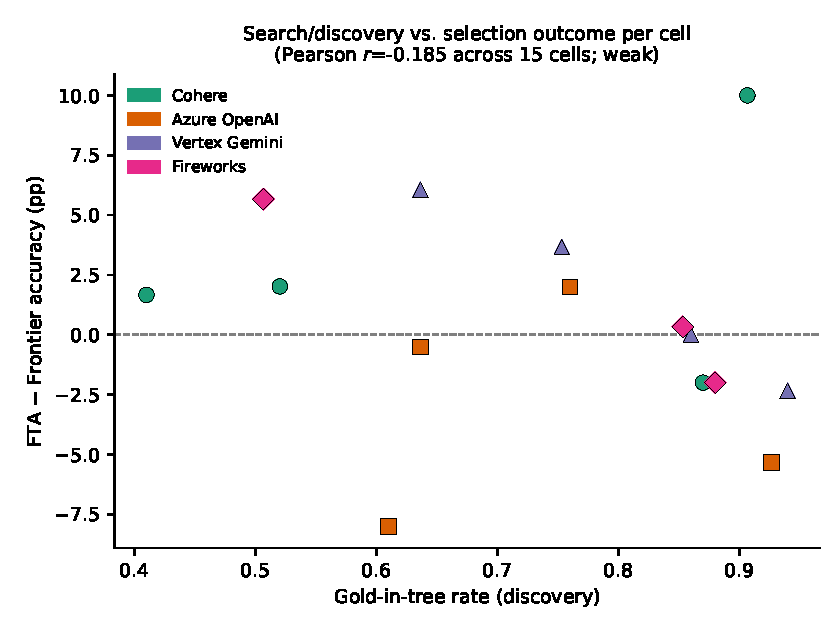
\includegraphics[width=0.78\linewidth]{figure3_search_vs_selection_scatter}
\caption{Discovery rate vs.\ FTA$-$Frontier delta (15 cells). Global Pearson $r=-0.185$ (not
supported at $n{=}15$); leave-one-out ranges vary. Descriptive sanity check; Azure sign reversal is
the clearer tested instance (Section~\ref{sec:provider-analysis}).}
\label{fig:scatter}
\end{figure}
